


\documentclass{rspublic}
\usepackage{graphicx}
\usepackage{epsfig}
\usepackage{epsf}
\usepackage{amssymb}
\usepackage{amsmath}
\usepackage{amsthm}
\usepackage{multirow}
\usepackage{hyperref}

\newcommand{\bra}[1]{\langle #1|}
\newcommand{\ket}[1]{|#1\rangle}

\newcommand{\be}{\begin{equation}}
\newcommand{\ee}{\end{equation}}
\newcommand{\bea}{\begin{eqnarray}}
\newcommand{\eea}{\end{eqnarray}}
\newcommand{\Fig}[1]{Fig.\,\ref{#1}}
\newcommand{\Eq}[1]{Eq.\,(\ref{#1})}
\newcommand{\la}{\langle}
\newcommand{\ra}{\rangle}
\newcommand{\nl}{\nonumber \\}
\usepackage[usenames]{color}
\definecolor{Red}{rgb}{1,0,0}
\definecolor{Blue}{rgb}{0,0,1}






%%%%%%%%%%%%%%%%% END OF PREAMBLE %%%%%%%%%%%%%%%%





% Include your paper's title here
\title{Experimental Study of the Quantum Simulation Towards Quantum Chemistry with an NMR Simulator
}

\shorttitle{Quantum Simulation}

\author{Dawei Lu$^{1}$, Nanyang Xu$^{1}$, Boruo Xu$^{2}$, Zhaokai Li$^{1}$, Hongwei Chen$^{1,3}$,  Xinhua Peng$^{1}$,  Ruixue Xu$^{1}$,  and Jiangfeng Du$^{1,\ast}$ }

\affiliation{$^{1}$Hefei National Laboratory for Physical Sciences at
Microscale and Department of Modern Physics, University of Science
and Technology of China, Hefei, Anhui, 230026, China, Email: djf@ustc.edu.cn\\
$^{2}$King's College, University of Cambridge, Cambridge CB2 1ST, United Kingdom\\
$^{3}$High Magnetic Field Laboratory, Hefei Institutes of Physical Science, Chinese Academy of Sciences, Hefei, Anhui, 230031, China
}






\begin{document}

\maketitle



\begin{abstract}

Quantum computers have been proved to be able to mimic quantum systems efficiently in polynomial time. Quantum chemistry problems, such as static molecular energy calculation and dynamical
chemical reaction simulation, become very intractable on classical computers with the system scaling up. Therefore, quantum simulation is a feasible and effective approach to tackle quantum chemistry problems.  Proof-of-principle experiments have been implemented on the calculation of the hydrogen molecular energies and the one-dimensional chemical isomerization reaction dynamics using nuclear magnetic resonance (NMR) systems. We conclude that quantum simulation will surpass the classical computers towards quantum chemistry in the near future.
\\

\footnotesize{\bf{Keywords: quantum simulation; quantum chemistry; nuclear magnetic resonance} }

\end{abstract}

\subsection{Introduction}

What type of computer can we utilize to simulate quantum systems? At least classical computer is not an affirmative choice. Although it can deal with tremendous common problems at present,
when the target system is quantum mechanical whose evolution obeys the Schr\"{o}dinger equation, classical computer is unfortunately failing. Suppose that the system size scales up and expands rapidly, the computational cost grows exponentially and soon it will exceed the capacity of any current computers. In 1982, Richard Feynman presented a path to solve this problem \cite{Feynman}, "...there is to be an \emph{exact} simulation, that the computer will do \emph{exactly} the same as nature.". The idea of quantum simulation, using controllable quantum systems to mimic other quantum systems, was suggested for the first time. Lloyd proved that universal quantum simulators can be built with quantum computation architecture, whose required resources scale polynomially with the size of the simulated system \cite{Lloyd}.

Compared to the quantum algorithms which, in general, requires thousands of qubits to excel the classical computing (e.g., Shor's quantum factorizing algorithm \cite{Shor}), a quantum simulator would realize with merely tens of qubits \cite{Buluta}. Moreover, quantum simulation is less demanding than quantum computing because, typically, it does not require either explicit quantum gates or error corrections. Furthermore, the level of coherent control technique of quantum systems necessary for
the physical realization of quantum simulation is now within reach \cite{Insight}. Therefore, quantum simulation is attracting plentiful interest in an enormous range of fields, including quantum chemistry, materials science, quantum many-body problems, condensed matter physics \emph{etc}. During the past few years several quantum simulation algorithms designed were
proposed, which were engineered for particular problems \cite{Zalka,Abrams,Wu,Smirnov,Lidar}. The pioneering experiments were first implemented in NMR systems. The first simulation was on quantum
oscillators \cite{Somaroo}, followed by quantum phase transition \cite{Peng}, quantum many-body problems \cite{Negrevergne} and a pairing Hamiltonian \cite{Yang,Brown}. Later, simulation of quantum phase transitions of a two-spin quantum magnet \cite{Friedenauer} and simulation of the Dirac equation \cite{Gerritsma} were performed using trapped ions. In this paper, our discussion is  focused on the issue of quantum simulation of quantum chemistry \cite{review}, essentially including experiments on the static molecular energies and dynamic chemical reactions.




\subsection{Simulating Molecular Ground State Energy}

In quantum chemistry, one of the most significant problems is how to calculate molecular energies, which is a fundamental problem in computational quantum chemistry. The resources required, on classical
computers, for a full simulation of the molecular system would accumulate exponentially with increasing number of atoms involved, limiting such full configuration interaction (FCI) calculations of molecular energies to simple molecules, diatomic and triatomic molecules \cite{Thogersen}. This limitation led to the development of several approximate methods in predicting chemical
properties for large systems, such as density functional theory (DFT) calculations. Despite these approximate methods can exhibit superiority in solving some problems, there are weakness associated with them. For instance, the DFT approach would fail for the systems involving long-range charge-transfer excited states \cite{Dreuw}. Thus, quantum chemistry desires a universal method, perhaps quantum simulation being a reliable choice.

The problem of solving a molecular ground state energy can be equally considered as how to calculate the lowest eigenvalue of the Schr\"{o}dinger equation, which contains a time-independent Hamiltonian. Although the classical computers can deal with certain molecules to a fixed accuracy, the desired resources would scale exponentially along with the size of of molecules and soon exceed the capacities of classical computers. In contrast, theoretically, quantum computers are able to simulate the ground state energy to the precision required by quantum chemistry, with just polynomial time complexity.
In 2005, Aspuru-Guzik \emph{et al}. proposed an algorithm to simulate a molecular system and to calculate the energies of molecules \cite{static}. The information of the
energy is coded in the phase shift of a quantum register, measured with a quantum phase estimation algorithm (PEA) \cite{Abrams,pea2}. The main process can be summarized into three steps (Fig. \ref{fig2}(a)):

\begin{figure}[htb]
\begin{center}
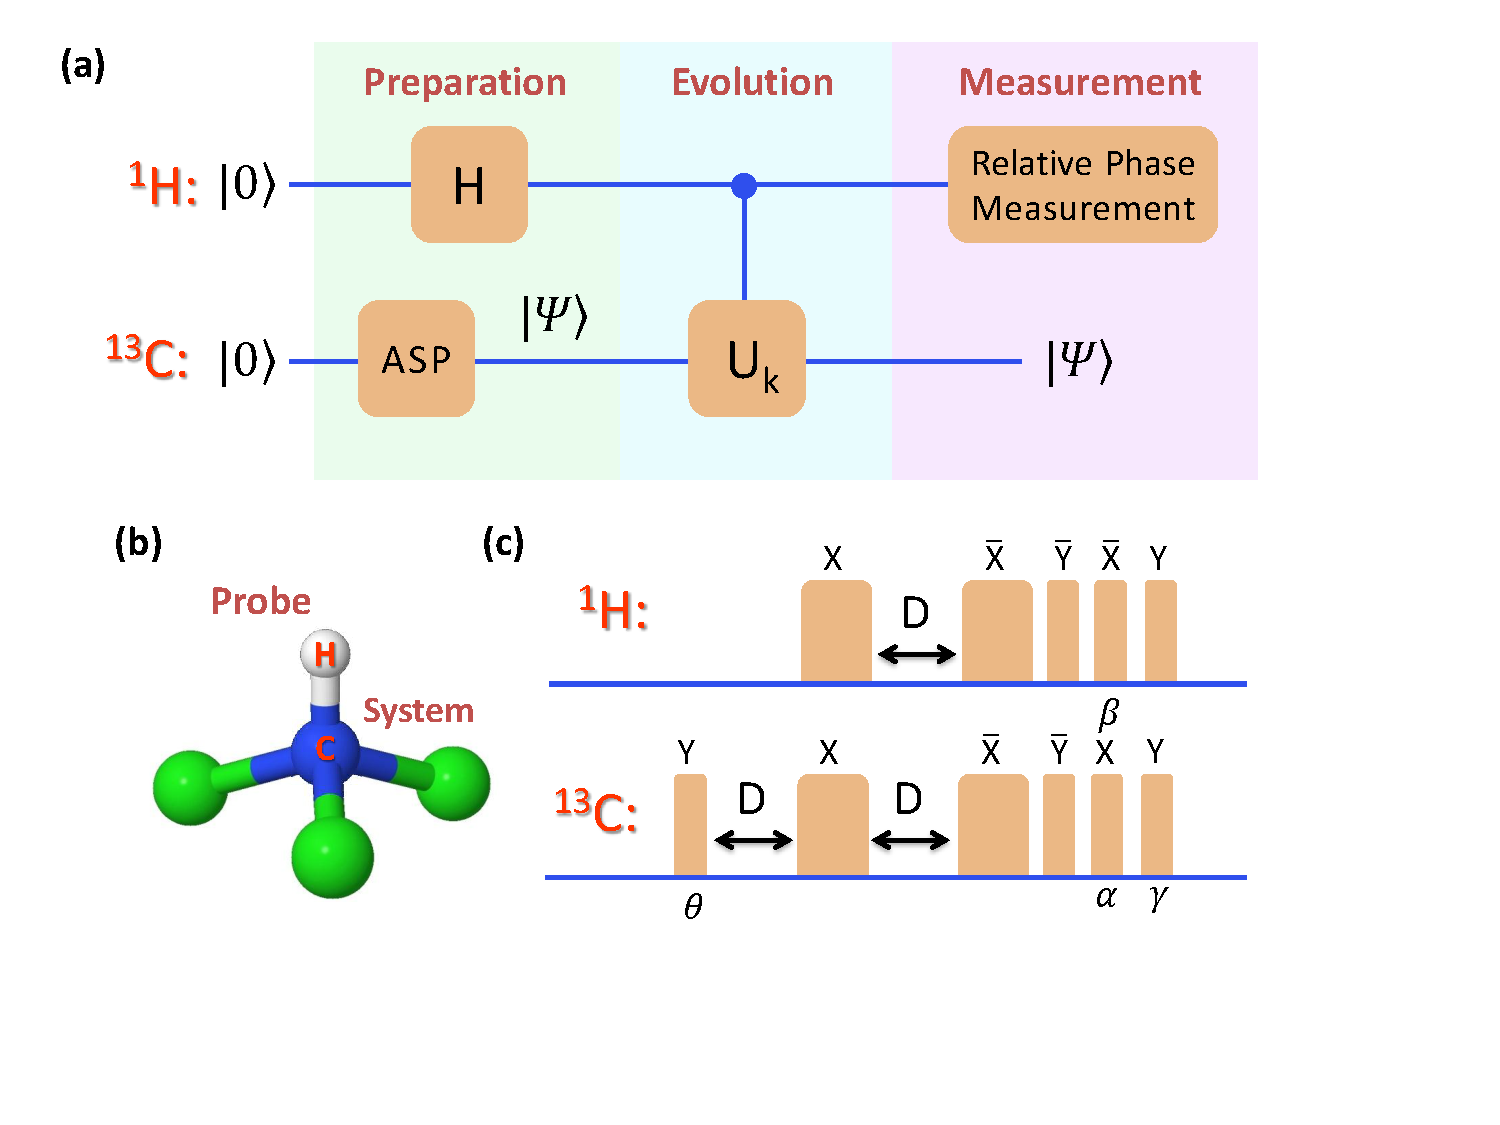
\includegraphics[width= 0.95\columnwidth]{fig2.eps}
\end{center}
\caption{\footnotesize{(color online). (a) Network for the calculation of the hydrogen molecular energies in our experiment.
(b) Molecular structure of the quantum register CHCl$_3$, with the system qubit $^{13}$C and the probe qubit $^{1}$H.
(c) Pulse sequence to implement
the controlled-$U_k$ operation, where $\theta =$ arctan$(\frac{2H(1,2)}{H(1,1)-H(2,2)})=0.226$, $\gamma = \frac{\pi}{2}-\theta=1.3458$, $\beta = \beta_k^0-\phi_{k-1}'$, $\alpha = \frac{8^{k-1}\tau}{2}\sqrt{4H(1,2)^2+(H(1,1)-H(2,2))^2}$ and $D=\frac{\alpha}{\pi J_{wa}}$ for the \emph{k}th iteration. Totally 15 iterations are performed in our experiment.}}\label{fig2}
\end{figure}

(a)\emph{Encoding}-Mapping the molecular wavefunction to the status of qubits. This initializing manipulation is the first step of almost all kinds of quantum simulation tasks, establishing a bridge between the physical system and the simulated system. Undoubtedly, the qubits needed grow with the size of the target molecule, and thus the method of preparing qubits to the ground state $\phi$ of the molecular Hamiltonian becomes more complicated.

(b)\emph{Evolution}-Simulating the time evolution of the molecular Hamiltonian. The goal of this step is to generate a phase shift on the probe qubit, which reflects the information of the eigenvalue of the ground state energy. The PEA indicates that, if we apply a unitary operator $U=e^{-iH\tau}$ on the ground state $\left\vert \psi \right\rangle$, a phase will be generated as $U \left\vert \psi \right\rangle = e^{-iH\tau}\left\vert \psi \right\rangle = e^{-iE\tau}\left\vert \psi \right\rangle = e^{i2 \pi \phi}\left\vert \psi \right\rangle$, where $E=-2\pi\phi/\tau$ is the energy of the ground state. Therefore, measurement of the phase is equivalent to calculating the ground state energy.

(c)\emph{Measurement}-Measuring the phase shift of the probe qubit, in order to get the value of the ground state energy. To fulfill this purpose, a four-bit inverse quantum Fourier transform (QFT) is adopted for the relative phase measurement, needing four qubits to obtain one precise bit with successful possibility of 15/16.


In the theoretical proposal, it is demonstrated that the number of qubits
required scales linearly with the number of basis functions, and the number of gates required grows polynomially with the number of qubits. Additionally, calculations of the
water and lithium hydride molecular ground-state energies were carried out on a quantum simulator using a recursive PEA.

Although this proposal is almost perfect in theory, examining such large molecules, i.e. water and lithium hydride, is unfeasible at the time of the experiment.
 When the system expands to a large Hilbert space, the current technology in quantum computing is difficult to support the requirements like the initial state preparation, the decomposition of the circuit, and the readout of the phase shift. As the first step of quantum simulation towards quantum chemistry, Lanyon \emph{et al.} \cite{static_exp1} and we \cite{static_exp2} both selected the simplest but significant scenario: simulating the ground state energy of Hydrogen molecule. In Lanyon's paper, a key step to the realization of the algorithm was carried out on a photonic system, and the ground state energy was calculated with a 20-bit precision. In our experiment, we chose a widely used STO-3G basis set in FCI \cite{Levine}, and obtained the ground state energy to a 45-bit precision using an NMR quantum simulator.

From the theory, adopting the Born-Oppenheimer approximation, the Hamiltonian of electron in the Hydrogen molecule can be described as \begin{eqnarray}\label{Hamiltonian}
\mathcal{H}=&&\sum\limits_{i=1}^2 (T_i+\sum\limits_{j=1}^2V_{ij})+\sum\limits_{i,j=1,i>j}^2O_{ij},
\end{eqnarray}
where $T_i$ is the kinetic energy of
the \emph{i}th electron, $V_{ij}$ is the Coulomb potential energy between the \emph{i}th electron and the \emph{j}th nucleus, and $O_{ij}$ is the Coulomb potential energy between the \emph{i}th electron and \emph{j}th electron. In this model, each atom has a 1\emph{s} Gaussian-type function in STO-3G basis, consisting one bonding orbital with gerade symmetry and one antibonding orbital with ungerade symmetry. This structure forms 4 spin orbits corresponding to 6 possible configurations. Furthermore, only two configurations contribute to the ground state energy calculation: the ground state configuration $|\Psi_0\rangle$ and
the double excitation configuration $|\Psi_{1\bar{1}}^{2\bar{2}}\rangle$. So the singlet symmetry and spatial symmetry of the ground state can be simplified. In atom units (a.u.), the nuclear distance $\gamma$ is 1.4 a.u., and the Hamiltonian of this model is \cite{Szabo}:
\begin{eqnarray}
        H&=&
        \begin{pmatrix}
            \langle\Psi_0|H|\Psi_0\rangle & \langle\Psi_{1\bar{1}}^{2\bar{2}}|H||\Psi_{1\bar{1}}^{2\bar{2}}\rangle\\
            \langle\Psi_{1\bar{1}}^{2\bar{2}}|H|\Psi_0\rangle & \langle\Psi_{1\bar{1}}^{2\bar{2}}|H|\Psi_{1\bar{1}}^{2\bar{2}}\rangle
            \end{pmatrix}\nonumber\\
        &=& \begin{pmatrix}
            -1.8310 & 0.1813\\
            0.1813 & -0.2537
            \end{pmatrix}
\end{eqnarray}
whose eigenvalue is -1.85157092935119 a.u.

To perform this simulation, we selected a 2-qubit NMR quantum simulator. Each qubit is represented by $^{13}$C (system qubit) and $^{1}$H (probe qubit)
nuclear spins in the $^{13}$C-labeled chloroform dissolved in $d_6$ acetone, respectively. The
molecular structure is shown in Fig. \ref{fig2}(b), where the
two qubits are marked. The internal Hamiltonian of this two-qubit
system is:
\begin{eqnarray}\label{HamCHF}
\mathcal{H}_{int}=\frac{\omega_{H}}{2}\sigma_{z}^H+\frac{\omega_{C}}{2}\sigma_{z}^{C}+\frac{\pi
J_{CH}}{2}\sigma_{z}^{H}\sigma_{z}^{C}
\end{eqnarray}
where $\omega_{H}/2\pi$ and $\omega_{C}2\pi$ are the Larmor
frequencies and $J_{CH}$ represents the weak coupling constant,
typically, $J_{CH}=214.6Hz$.

The whole experiment can be divided into three sections: (i) the adiabatic preparation of the system qubit $^{13}$C to the ground state of the Hamiltonian; (ii) the application of the time evolution of the Hamiltonian on the qubits to generate the phase shift on the probe qubit; (iii) measurement of the phase shift on the qubit to extract the energy information. Now, we will discuss these three parts in details.

(i) \emph{Initial state preparation.} The thermal equilibrium state is a mixed state, which is not suitable for most quantum simulating tasks. Therefore we fist create a pseudopure state (PPS) $\rho_{00} =\frac{1 -
\epsilon}{4} \mathbf{I}+ \epsilon|00\rangle \langle 00|$ using the
spatial average technique \cite{spatial}, with $\mathbf{I}$
representing the $4 \times 4$ unity operator and $\epsilon \approx
10^{-5}$ the polarization. Then we prepared the system qubit to the ground state $|\Psi\rangle$ through the adiabatic state preparation (ASP) process, and the probe qubit to the state $|+\rangle=\frac{1}{\sqrt{2}}(|0\rangle+|1\rangle)$ by a pseudo-Hadamard gate $R_{y}^{H}
(\pi/2)$.

To prepare the ground state $|\Psi\rangle$, ASP method based on the quantum adiabatic theorem \cite{adiabatic} is a simple and accurate approach. Besides, the adiabatic computational model has been proposed \cite{Farhi} and has been proven equivalent to the conventional circuit model \cite{Mizel}. The quantum adiabatic theorem states that, a quantum system remains in its instantaneous eigenstate if the system Hamiltonian varies slowly enough and if there is a gap
between this eigenvalue and the rest of the Hamiltonian's spectrum \cite{adiabatic}. Applying this technique we drove the qubits from the ground state of a simple Hamiltonian $H_0 = \sigma _x$ to the target by varying the system Hamiltonian sufficiently slowly.  The system qubit is prepared into the ground state $|-\rangle=\frac{1}{\sqrt{2}}(|0\rangle-|1\rangle)$ of $H_0$ by a conjugated pseudo-Hadamard gate $R_{y}^{H}
(-\pi/2)$. The slow-varying discrete Hamiltonian is interpolated from a linear form $H_{ad}=(1-s)\sigma_x + sH$
with $s=\frac{t}{T}$. The success of ASP is ensured by T = 5.52 a.u. yielding from the numerical simulation \cite{Steffen,Liao}.  Thus the unitary operator for each adiabatic step using Trotters' formula is
\begin{equation}
U_{m}=e^{-i\frac{\delta t}{2}(1-s_m)\sigma_{x}}e^{-is_mH\delta t}
e^{-i\frac{\delta t}{2}(1-s_m)\sigma_{x} }+O({\delta t}^{3}),
\end{equation}
where the duration $\delta t = T/(M+1)$ and $s_m=m/(M+1)$. A simple sequence including three single-rotating pulses $R_{-x}^{C}(\theta_{1})-R_{-y}^{C}(\theta_{2})-R_{x}^{C}(\theta_{3})$ can implement $U_m$ directly, and the total evolution can be realized by repeating this sequence consequently. So far we have completed the preparation of the initial state.

(ii) \emph{Time evolution.} In this step we will introduce two techniques first: the NMR interferometer \cite{inter1,inter2} and the iterative scheme, followed by the implementation of the methods.

In the theoretical proposal mentioned above, a four-bit QFT is essential for evaluating the phase shift. However, in our case, in NMR system the relative phase was readout by an NMR interferometer, whose principle is very similar to the interferometer in optics. This device is a sensitive detector and more precise than the original four-bit QFT
gate as the error bound of the phase shift measured is less than
$\pm 5^{\circ}$. As well, the theory ensures that arbitrary precision can be achieved using the iterative process. The initial condition was $U_0=U$ and the iterative form was selected as $U_{k+1}=[e^{-i2\pi\phi_k'}U_k]^{2^n}$, where $n$ is the number of bits and $\phi_k'=max\{\phi_k-\phi_{errbd}, 0\}$.

The controlled-rotating gate (represent by the solid dot) functions as the following: when the control qubit $^1$H is $|0\rangle$, the system $^{13}$C remains unchanged, and when the control qubit is $|1\rangle$, the system undergoes the $U_k$ evolution. Thus the operator can be described as
\begin{equation}
C_{U_k}=|0\rangle\langle 0|\otimes I +|1\rangle\langle 1|\otimes U_k.
\end{equation}
Applying $U_0=e^{-iH\tau}$, the initial state $|\psi_{in}\rangle=\frac{1}{\sqrt{2}}(|0\rangle+|1\rangle)|\Psi\rangle$ transformed into
\begin{equation}
|\psi_{ifm}\rangle=\frac{1}{\sqrt{2}}(|0\rangle+e^{i2\pi\phi}|1\rangle)|\Psi\rangle.
\end{equation}
The relative shift can be readout directly in NMR with this interferometer. Here the evolution time is
\begin{equation}
\tau = [\pi/\sqrt{(2H(1,2))^2+(H(1,1)-H(2,2))^2}].
\end{equation}
The pulse sequence for conducting $C_{U_k}$ is shown in Fig. \ref{fig2}(c).

(iii) \emph{Phase measurement.} After each iteration, we measured the phase shift and thereby adjusted the operator for the next iteration using the scheme described before. The quadrature detection in NMR serves as a phase detector. If the initial state is set as the reference phase, all the relative phases can be readout directly in the NMR spectra. Additionally, the value $\phi_k'$ in each iteration is stored for further use. After measuring all the 15 phases, we use a recursive method to rebuild $\phi$ as the experimental result, formulated as,
\begin{equation}
\phi_i^{result} = \phi_{i+1}^{result}/\phi_{errbd}+\phi_i',
\end{equation}
where $\phi_{i+1}^{result}$ is merely the intermediate value with no physical meaning. Finally we get the experimental result, which approaches the theoretical value of $\phi$. In 15 iterations the eigenvalue of the molecular Hamiltonian is extracted as -1.851570929351124, and the intermediate result after each iteration is shown in Fig. \ref{fig3}.

\begin{figure}[htb]
\begin{center}
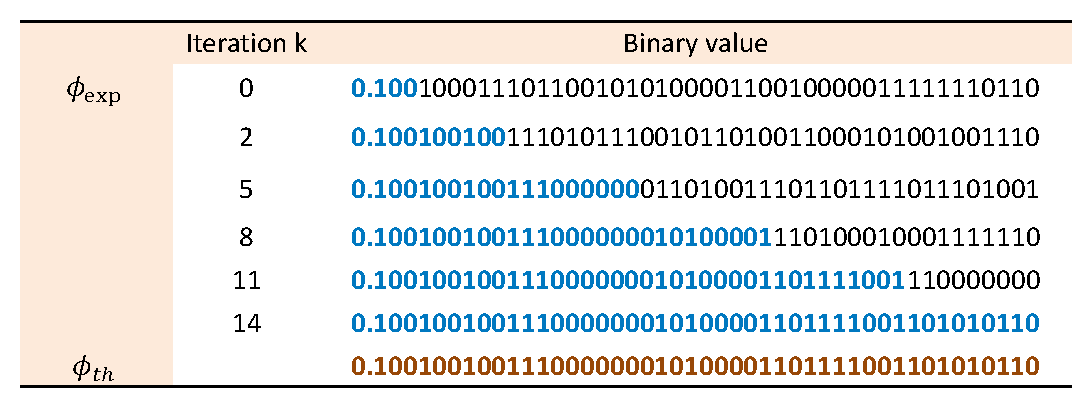
\includegraphics[width= 0.95\columnwidth]{fig3.eps}
\end{center}
\caption{\footnotesize{(color online). Experimental $\phi$ values ($\phi_{exp}$) measured in iterations, compared to the theoretical
expectation $\phi_{th}$. The numbers in bold are the bits obtained from the experiment, where 3 bits are
extracted in each iteration. Through 15 iterations, we ultimately obtained 45 bits of $\phi$.}}\label{fig3}
\end{figure}

To conclude, we simulate the hydrogen molecule and calculate the ground state energy of it to a precision of 45 bits in our NMR quantum
simulator. These two experiments \cite{static_exp1,static_exp2} are significant progress towards the goal of achieving a rapid quantum chemistry simulation. In terms of the scalabilities,, the main issues are the efficient decomposition of the evolution operator \cite{static_exp1} and the complexity of the adiabatic passage \cite{Young}, both of which are are at least feasible on medium molecular sizes. It is foreseeable that, with the confronted technical challenges overcome gradually, a quantum simulator is expected to speed up quantum chemistry calculations on a medium scale quantum computer.

\subsection{Simulating Chemical Isomerization Reaction Dynamics}

\begin{figure}[htb]
\begin{center}
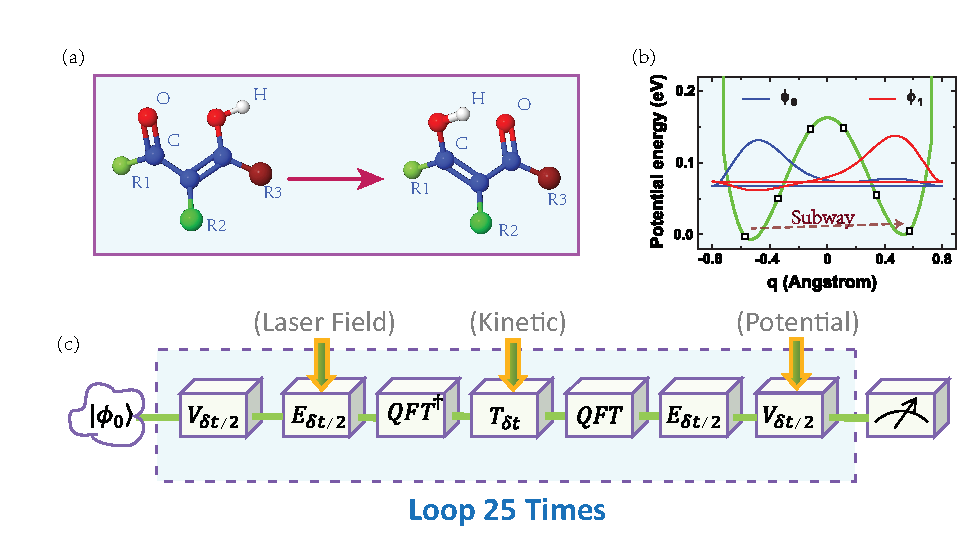
\includegraphics[width= 0.95\columnwidth]{fig4.eps}
\end{center}
\caption{\footnotesize{(color online). (a) Isomerization reaction of nonsymmetric substituted malonaldehydes.
(b) Potential energy curve, together with the eigenfunctions of
    the ground (blue) and the first excited (red) states.
(c) Network of quantum operations to simulate the isomerization dynamics, with the reactant state $\left\vert \phi_{0} \right\rangle$.
The whole process is divided into 25 loops. The operators $T_{\delta t}$, $V_{\delta t}$ and $E_{\delta t/2}$ are assumed to be in their
diagonal representations.
    }}\label{fig4}
\end{figure}

We have discussed an implementation of quantum simulation of a static chemical model in the previous section. Now our interests have turned to quantum simulation of a dynamic chemical process. Classical computers have achieved remarkably at simulating small quantum chemical system, though, assisted by Born-Oppenheimer approximation and various techniques \cite{Manthe,WuYH,Ben}, these methods have reduced the originally exponentially cost problem to a polynomial one, at given accuracy. However, Ivan Kassal \emph{et al.} in 2008 proposed an algorithm \cite{Kassal} illustrating that quantum chemical reaction simulations can be done universally in polynomial time complexity without approximations.  In this algorithm, they introduced ancillary qubits to the procedure, for the ease of decomposing operators into elementary quantum gates, when the system scales up to more than a few qubits.  Also they iterated the process to improve the accuracy of the quantity of interest. Furthermore, they demonstrated that simulating  the entire electronic and nuclear interaction evolving in time is more effective than applying the Born-Oppenheimer approximation for a quantum computer, comparing to classical computers, provided that the chemical reactions invlove more than 4 atoms.

Based on their algorithm, we experimentally realized the quantum simulation of a chemical isomerization reaction using an NMR quantum simulator \cite{Dawei}. In particular, we testified a one-dimentional model of the reaction, driven by a laser, of relocating hydrogen on non-symmetric substituted malonaldehydes \cite{subway} shown in Fig. \ref{fig4}(a). In this model, a method, namely "hydrogen-subway", used low intensities of laser to avoid Keldysh limit \cite{Keldysh}, which is a potential problem in conventional above barrier pump-dump approach involving high intensities laser fields, provided that both methods achieving same percentage of product yields (Fig. \ref{fig4}(b)).



\begin{figure}[htb]
\begin{center}
\includegraphics[width= 0.95\columnwidth]{fig5.eps}
\end{center}
\setlength{\abovecaptionskip}{-5.35cm}
\caption{\footnotesize{(color online). (a) Molecular structure of Diethyl-fluoromalonate and the system parameters.
The $^1$H, $^{13}$C and $^{19}$F nuclear spins marked by oval are used as three qubits.
Diagonal elements are the Larmor frequencies (Hz) and
off-diagonal elements are scalar coupling strength (Hz) between two nuclear spins.
Relaxation and dephasing time scales (second) $T_1$ and $T_2$ for each nuclear spin are listed on the right.
(b)Measured probabilities of the reactant and product states to give 25 snapshots of the reaction dynamics.   The (red) plus symbols represent measured results of the percentage of the reactant in the intermediate product, and the (blue) circles represent measured results of percentage of the final product in the intermediate product, both in agreement with the theoretical smooth curves.}}\label{fig5}
\end{figure}

The experiment is accomplished on a Bruker Avance 400 MHz spectrometer at room temperature. Qubits 1,2, and 3 are realized by the $^{19}$F, $^{13}$C, and $^1$H nuclear spins of Diethyl-fluoromalonate.  The structure of Diethyl-fluoromalonate is shown in Fig. \ref{fig5}(a), where the three nuclei used as qubits are marked by an oval. The internal Hamiltonian of this system is given by
\begin{eqnarray}\label{Hamiltonian}
\mathcal{H}_{int}=&&\sum\limits_{j=1}^3 {2\pi \nu _j } I_z^j  + \sum\limits_{j < k,=1}^3 {2\pi} J_{jk} I_z^j I_z^k,
\end{eqnarray}
where $\nu_j$ is the resonance frequency of the \emph{j}th spin and
$\emph{J}_{jk}$ is the scalar coupling strength between spins \emph{j} and
\emph{k}.

In our experiment, we would conduct the process in the following steps: preparing the molecule into the desired initial state, followed by evolving it with time and then taking measurements during and after the experiment. Starting from the originally time independent Hamiltonian system operator, we modified it by adding the external laser field into consideration,
\begin{equation}\label{totH}
  H(t)=  T+  V+  E(t) { \quad   \rm  with   \quad    }
                            E(t)=- \mu\varepsilon(t).
\end{equation}
where T and V are kinetic and potential energy operator respectively and E(t) is the contributing term from the laser operation.  Additionally T and V solely depend on positions and the latter takes the form of a double-well potential of the system. Thus E(t), the time varying laser-molecule interaction Hamiltonian offered  "hydrogen-subway" approach, enabling  the reaction to occur while the energy of the molecule below the barrier height \cite{subway}.

Due to the asymmetry of the two wells, we assumed that the initial reactant state is the ground state of the system and is primarily localised in the left potential well shown in Fig. \ref{fig4}(b). The corresponding product state is taken as being chiefly localized in the right potential well, which is expected to be the first excited state of T + V.
For the purpose of preparing our chemical molecule into the initial state, the state under the bare Hamiltonian T + V, in practice, we created a pseudo state from the thermal equilibrium state, which was then applied with a pre-set radio-frequency (rf) pulse, determined by GRadient Ascent Pulse Engineering (GRAPE) algorithm \cite{grape1,grape2,grape3}. At the end of the procedure, in order to confirm that the molecule was in the reactant state, from a full state tomography and a fidelity test, we acquired results indicating a strong agreement between the theoretical initial state and the prepared state (Fig. \ref{fig6}(a)).

Now we have obtained our initial wave function for the molecule, we would like to evolve it in time. In another word, we applied the propagator of Hamiltonian operator to the function, labeled as $U_m$, $U(\delta t)=e^{-iH\delta t}$, where H followed the definition in Eq.
\ref{totH}. Here we quantized V, the potential well, with 8 discrete points, corresponding to 3 qubits. Also since it is tremendously difficult to implement the propagator operator directly, we used the Trotter formula \cite{Trotter} to decompose the propagator into a simpler form,
\begin{align}\label{propagator}
 {U}(t+\delta t,t)\approx &\,
 e^{-\frac{i}{\hbar} {V} \delta t/2} e^{-\frac{i}{\hbar} {E} (t+\delta t/2)  \delta t/2}
 e^{-\frac{i}{\hbar} {T} \delta t}   \nl & \times e^{-\frac{i}{\hbar} {E} (t+\delta t/2)           \delta t/2}
 e^{-\frac{i}{\hbar} {V} \delta t/2} .
\end{align}
where the propagator $ {U}(t+\delta t,t)$  was related to the time interval between t to $\delta t$. Therefore we decomposed it into unitary diagonal operators in either the position or momentum representation, which were associated into one coordinate system by executing QFT to one of the representations \cite{Coppersmith}, in this case, to the momentum one. Thus, $U_m$ could be emulated in a simple manner, since decomposed components were all unitary and diagonal in position representation, and one loop was accomplished by completing all these operators in order as shown in Fig. \ref{fig4}(c), with a rf pulse sequence.

Indeed, we could obtain the same result by introducing ancilla, but that would require extra qubits which were not available at the time of the experiment. Instead, we turned to the GRAPE approach, effective and successful on the NMR simulator with low dimensions of state functions. However, at high dimension of density matrix, the wave function, ancilla provides a feasible solution to decompose the unitary operator, U, into simple additions and other arithmetical operations.

Besides, iterating this procedure would improve the accuracy of the final result. We, in practice, repeated the process 25 times, and the number of iterations was limited by the decoherence time of the NMR system and the operation time of implementing each operator by applying rf pulses. In order to push to the limit of precision, we combined the individual rf pulse for each operator in one loop, into one single rf pulse with high fidelities using GRAPE, which is a facile task on a 3-qubit system, and thus reduces the technical complexity of the experiment and the overall operation time, avoiding additional experimental errors and severe decoherence effects. Consequently we reached highly accurate outcomes without losing fidelities.
Between the iterations, we measured the overlap between the density matrix and that of the theoretical initial state and the final state, respectively, to perceive the transition from the reactant to the product. Although the measurements could be achieved with full state tomographies, the information we were interested in was extracted by population measurements, with aid of a simple diagonalization technique, simplifying the experiment and reducing the required resources.

\begin{figure}[htb]
\begin{center}
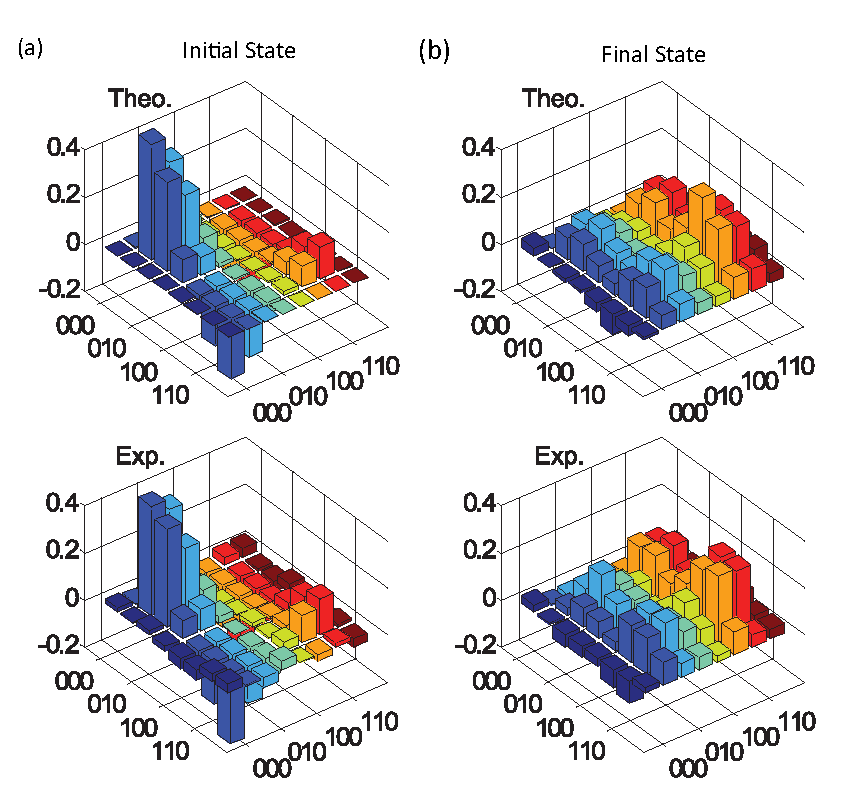
\includegraphics[width= 0.95\columnwidth]{fig6.eps}
\end{center}
\caption{\footnotesize{(color online). (a)-(b) Real part of the density matrix of the initial and final states of the simulated reaction.
Upper panels show the theoretical results based on an 8-dimensional Hilbert space, and lower panels show the experimental results.}}\label{fig6}
\end{figure}



In addition, we would like to examine the difference between theory and experiment for the final result. By applying a full state tomography to the final state density matrix at the end of the iterations, the experimental density matrix was found to be agreed with the theoretical one acquired in an eight dimensional Hilbert space to a great degree, as shown in Fig. \ref{fig6}(b), with a high fidelity of 0.957 out of 1, which was resulting from the high fidelity of the GRAPE pulse. Furthermore, the experimental density matrix elements of the final state matched the theoretical results remarkably.
Thus simulated reaction dynamics can be studied by inspecting the probabilities of being in the reactant and product states respectively through the reaction, given the confidence on the experimental outcomes on the full density matrix level. Fig. \ref{fig5}(b) illustrates the time dependence of the probabilities of being in either state attained from our quantum simulator. From the graph, the product-to-reactant ratio grows continuously with respect to time, with 77\% possibilities of product state when the simulation terminated.

As a result, our 3-qubit system positively simulated a prototype laser-driven chemical reaction. Additionally, we point out that the spin decoherence time of our system is significantly longer than our simulation experiment, in particular, 30ms, which is due to combining the gate operations, GRAPE pulses, and thus is due to the reduction of the number of operations.  Further, few sources could contributed to the minor discrepancy between the theory and the experiment, for instance, the unfaithfulness of GRAPE pulses, the inhomogeneity in rf pulses and in the static magnetic field.

\subsection{Conclusion}

Quantum simulation provides a huge prospect in quantum chemistry in terms of static molecule modeling and dynamic reaction simulation. Our proof-of-principle experiments verified those two points for simple molecules and reactions. However, with only a few tens of qubits, quantum simulation could reach beyond the limit of classical computing \cite{static}, i.e. simulating large molecules or complex reactions. This could be achieved when technical barriers are overcome, which occur in mapping eigenstates into qubits and decomposing the molecular evolution operator into quantum logic gates. In NMR systems, one method to encode the initial eigenstate into qubits is via adiabatic state preparation. However, this has problems when system scales up as calculating a conclusive mathematical analysis is hard at the moment. Nevertheless, progress has been made in this area, the scalability of NMR quantum computer \cite{Young}, and it is foreseeable that quantum simulation would have practical use for medium size molecules and reactions.

\subsection{Acknowledgement}
This work was supported by National Nature Science Foundation of China (Grants No. 10834005, No. 91021005, and No. 21073171), the CAS, and the National Fundamental Research Program 2007CB925200.






\begin{enumerate}
\bibitem{Feynman} Feynman, R. P. 1982 Simulating physics with computers. {\it Int. J. Theor. Phys.} \textbf{21}, 467. (doi: 10.1007/BF02650179)
\bibitem{Lloyd} Lloyd, S. 1996 Universal quantum simulators. {\it Science }\textbf{273}, 1073. (doi:10.1126/science.273.5278.1073)
\bibitem{Shor} Shor, P. 1994 {\it Proceedings of the 35th annual symposium on foundations of computer science} (IEEE Computer Society Press, New York, Santa Fe, NM, ), p. 124. (doi:10.1109/SFCS.1994.365747)
\bibitem{Buluta} Buluta, I. \& Nori, F. 2009  Quantum simulators. {\it Science} \textbf{326}, 108.(doi: 10.1126/science.1177838 )
\bibitem{Insight} Vedral, V. \emph{et al}. 2008 Natureinsight: Quantum coherence. {\it Nature.} \textbf{453}, 1003�C1049. (doi:10.1038/4531003a)
\bibitem{Zalka} Zalka, C. 1996 {\it ITP Conference on quantum coherence and decoherence}.(Royal Soc. London, Santa Barbara, California, ), pp. 313-322.
\bibitem{Abrams} Abrams, D. S. \& Lloyd, S. 1997 Simulation of many-body fermi systems on a universal quantum computer. {\it Phys. Rev. Lett}. \textbf{79}, 2586. (doi:10.1103/PhysRevLett.79.2586)
\bibitem{Wu} Wu, L. A., Byrd, M. S. \& Lidar, D. A. 2002 Polynomial-time simulation of pairing models on a quantum computer. {\it Phys. Rev. Lett.} \textbf{89},057904. (doi:10.1103/PhysRevLett.89.057904)
\bibitem{Smirnov} Smirnov, A. Y. \emph{et al.} 2007 Polynomial-time quantum algorithm for the simulation of chemical dynamics. {\it Europhys. Lett.} \textbf{80}, 67008. (doi: 10.1209/0295-5075/80/67008)
\bibitem{Lidar} Lidar, D. A. \& Wang, H. 1999 Calculating the thermal rate constant with exponential speedup on a quantum computer. {\it Phys. Rev. E} \textbf{59}, 2429. (doi:10.1103/PhysRevE.59.2429)
\bibitem{Somaroo} Somaroo, S., Tseng, C. H., Havel, T. F., Laflamme, R. \& Cory, D. G. 1999 Quantum simulations on a quantum computer. {\it Phys. Rev. Lett.} \textbf{82}, 5381. (doi:10.1103/PhysRevLett.82.5381)
\bibitem{Peng} Peng, X. H., Du, J. F. \& Suter, D. 2005 Quantum phase transition of ground-state entanglement in a Heisenberg spin chain simulated in an NMR quantum computer. {\it Phys. Rev. A} \textbf{71},012307. (doi:10.1103/PhysRevA.71.012307)
\bibitem{Negrevergne} Negrevergne, C., Somma, R., Ortiz, G., Knill, E. \& Laflamme, R. 2005 Liquid-state NMR simulations of quantum many-body problems. {\it Phys. Rev. A} \textbf{71}, 032344. (doi:10.1103/PhysRevA.71.032344)
\bibitem{Yang} Yang, X., Wang, A. M., Xu, F. \& Du. J. 2006 Experimental simulation of a pairing Hamiltonian on an NMR quantum computer. {\it Chem. Phys. Lett.} \textbf{422}, 20. (doi:10.1016/j.cplett.2006.02.023)
\bibitem{Brown} Brown, K. R., Clark, R. J. \& Chuang, I. L. 2006 Limitations of quantum simulation examined by simulating a pairing Hamiltonian using nuclear magnetic
resonance. {\it Phys. Rev. Lett.} \textbf{97}, 050504.
(doi:10.1103/PhysRevLett.97.050504)
\bibitem{Friedenauer} Friedenauer, A., Schmitz, H., Glueckert, J. T., Porras, D. \& Schaetz, T. 2008 Simulating a quantum magnet with trapped ions. {\it Nature Phys.} \textbf{4}, 757. ( doi:10.1038/nphys1032)
\bibitem{Gerritsma} Gerritsma, R.\emph{ et al.} 2010 Quantum simulation of the Dirac equation. {\it Nature.}\textbf{463}, 68. (doi:10.1038/nature08688)
\bibitem{Thogersen} Thogersen, L. \& Olsen, J. 2004 A coupled cluster and full configuration interaction study of CN and $CN^-$. {\it Chem. Phys. Lett.} \textbf{393}, 36. (doi:10.1016/j.cplett.2004.06.001 )
\bibitem{Dreuw} Dreuw, A. \& Head-Gordon, M. 2004 Failure of time-dependent density functional theory for long-range charge-transfer excited states: The zincbacteriochlorin-
bacterlochlorin and bacteriochlorophyll-spheroidene complexes. {\it
J. Am. Chem. Soc.}\textbf{126}, 4007�C4016. (doi: 10.1021/ja039556n)
\bibitem{static} Aspuru-Guzik, A., Dutoi, A. D., Love, P. J. \& Head-Gordon, M. 2005 Simulated quantum computation of molecular energies. {\it Science} \textbf{309}, 1704. (doi: 10.1126/science.1113479 )
\bibitem{pea2} Abrams, D. S. \& Lloyd, S. 1999 Quantum algorithm providing exponential speed increase for finding eigenvalues and eigenvectors. {\it Phys. Rev. Lett.} \textbf{83}, 5162. (doi:10.1103/PhysRevLett.83.5162)
\bibitem{review} Kassal, I., Whitfield, J. D., Ortiz, A. P., Yung, M. H. \& Aspuru-Guzik. A. 2011 Simulating chemistry using quantum computers. {\it Annual Review of Physical Chemistry.} \textbf{62}, 185-207. (doi: 10.1146/annurev-physchem-032210-103512)
\bibitem{static_exp1} Lanyon, B. P. \emph{et al.} 2010 Towards quantum chemistry on a quantum computer. {\it Nature Chem.} \textbf{2}, 106. (doi:10.1038/nchem.483 )
\bibitem{static_exp2} Du, J. F. \emph{et al.} 2010 NMR implementation of a molecular hydrogen quantum simulation with adiabatic state preparation. {\it Phys. Rev. Lett.} \textbf{104}, 030502. (doi:10.1103/PhysRevLett.104.030502)
\bibitem{Levine} Levine, I. N. 2000 Quantum chemistry (Prentice-Hall, Inc.,
Upper Saddle River, NJ), 5th ed.
\bibitem{Szabo} Szabo, A. \& Ostlund, N. S. 1996 Modern quantum chemistry
(Dover Publications, Inc., New York).
\bibitem{spatial} Cory, D. G., Fahmy, A. F. \& Havel, T. F. 1997 Ensemble quantum computing by NMR spectroscopy. {\it Proc. Natl. Acad. Sci. U.S.A.} \textbf{94}, 1634.
\bibitem{adiabatic} Messiah, A. 1976 Quantum mechanics (Wiley, New York,
); Kato, T. 1950 On the adiabatic theorem of quantum mechanics. {\it J. Phys. Soc. Jpn.} \textbf{5}, 435. (doi: 0.1143/JPSJ.5.435)
\bibitem{Farhi} Farhi, E. \emph{et al.}, 2001 Quantum adiabatic evolution algorithm applied to random instances of an NP-complete problem. {\it Science} \textbf{292}, 472. (doi: 10.1126/science.1057726)
\bibitem{Mizel} Mizel, A., Lidar, D. A. \& Mitchell, M. 2007 Simple Proof of Equivalence between Adiabatic Quantum Computation and the Circuit Model {\it Phys. Rev. Lett.}
\textbf{99}, 070502. (doi:10.1103/PhysRevLett.99.
070502)
\bibitem{Steffen} Steffen, M., van Dam, W., Hogg, T., Breyta, G., \& Chuang, I. 2003 Experimental implementation of an adiabatic quantum optimization algorithm. {\it Phys. Rev. Lett.} \textbf{90}, 067903. (doi:10.1103/PhysRevLett.90.067903)
\bibitem{Liao} Peng, X. H., Liao, Z. Y., Xu, N. Y., Qin, G., Zhou, X. Y., Suter, D., \&  Du, J. F. 2008 Quantum adiabatic algorithm for factorization and its experimental implementation. {\it Phys. Rev. Lett.} \textbf{101}, 220405. (doi:10.1103/PhysRevLett.101.220405)
\bibitem{inter1} Du, J. F., Zou, P., Shi, M. J., Kwek, L. C., Pan, J. W., Oh, C. H., Ekert, A., Oi, D. K. L., \& Ericsson, M., 2003 Observation of geometric phases for mixed states using NMR interferometry. {\it Phys. Rev. Lett.} \textbf{91}, 100403. (doi:10.1103/PhysRevLett.91.100403)
\bibitem{inter2} Peng, X. H., Zhu, X. W., Suter, D., Du, J. F., Liu, M. L., \& Gao, K. L. 2005 Quantification of complementarity in
multiqubit systems. {\it Phys. Rev. A.} \textbf{72},
052109. (doi:10.1103/PhysRevA.72.052109)
\bibitem{Young} Young, A. P., Knysh, S., \& Smelyanskiy, V. N., 2005 Evolution of entanglement between distinguishable light states. {\it Phys. Rev.
Lett.} \textbf{101}, 170503. (doi:10.1103/PhysRevLett.101.170501)
\bibitem{Kassal} Kassal, I. \emph{et al.} 2008 Polynomial-time quantum algorithm for the simulation of chemical dynamics. {\it Proc. Natl. Acad. Sci. U.S.A.} \textbf{105}, 18
681. (doi:10.1073/pnas.0802815105)
\bibitem{Manthe} Manthe, U., Meyer, H. -D., Cederbaum, L. S.,1992 Wave-packet dynamics within the multiconfiguration
hartree framework: General aspects and application to NOCl. {\it J.
Chem. Phys. } \textbf{97}, 3199-3213. (doi:10.1063/1.463007)
\bibitem{WuYH} Wu, Y. H., Batista, V. S., 2003 Matching-pursuit for simulations of quantum processes. {\it J. Chem.
Phys.} \textbf{118}, 6720-6724. (doi:10.1063/1.1560636)
\bibitem{Ben} Ben-Nun, M., \& Martinez T. J., 1998 Nonadiabatic molecular dynamics: Validation of the
multiple spawning method for a multidimensional problem. {\it J. Chem.
Phys. }\textbf{108}, 7244- 7257. (doi:10.1063/1.476142)
\bibitem{Dawei} Lu, D. W., Xu, N. Y., Xu, R. X., Chen, H. W., Gong, J. B., Peng, X. H., \& Du, J. F., 2011 Simulation of chemical isomerization reaction dynamics on a NMR quantum simulator
{\it Phys. Rev. Lett.} \textbf{107}, 020501. (doi:10.1103/PhysRevLett.107.020501)
%?
\bibitem{subway} {Do\v{s}li\'{c}}, N., K\"{u}hn, O., Manz, J. \& Sundermann K. 1998 The ��Hydrogen-Subway�� a tunneling approach to intramolecular hydrogen transfer reactions controlled by ultrashort laser pulses. {\it J. Phys. Chem. A,} \textbf{102}, 9645-9650 (doi: 10.1021/jp982470+)
%?
\bibitem{Keldysh} Keldysh, L. V. 1965 {\it SoV. Phys. JETP} \textbf{20}, 1307.
\bibitem{grape1} Khaneja, N., Reiss, T., Kehlet, C., Schulte-Herbr��ggen, T., \& Glaser, S. J. 2005 Optimal control of coupled spin dynamics: design of NMR pulse sequences by gradient ascent algorithms. {\it J. Magn. Reson.} \textbf{172}, 296. (doi:10.1016/j.jmr.2004.11.004)
\bibitem{grape2} Baugh, J. \emph{et al.}, 2007 {\it Phys. Canada} \textbf{63}, 4.
\bibitem{grape3} Ryan, C. A., Negrevergne, C., Laforest, M., Knill, E., \& Laflamme, R. 2008 Liquid-state nuclear magnetic resonance as a testbed for developing quantum control methods  {\it Phys. Rev. A} \textbf{78}, 012328. (doi:10.1103/PhysRevA.78.012328).
\bibitem{Trotter} Zalk, C. 1998 Simulating quantum systems on a quantum computer. {\it Proc. R. Soc. Lond. A} \textbf{454}, 313-322. (doi: 10.1098/rspa.1998.0162)
%1969??
\bibitem{Coppersmith} Coppersmith, D. 2002 An approximate fourier transform useful in quantum factoring.
arXiv:quant-ph/0201067.
\end{enumerate}


\end{document}
